\documentclass[11pt]{article}
% Preamble - Shared packages and macros

% Page geometry
\usepackage[margin=1in]{geometry}

% Math packages
\usepackage{amsmath}
\usepackage{amssymb}
\usepackage{amsthm}

% Graphics and figures
\usepackage{graphicx}
\usepackage{subcaption}
\usepackage{float}
\graphicspath{{figures/}}

% Tables
\usepackage{booktabs}
\usepackage{multirow}
\usepackage{array}

% Algorithms
\usepackage{algorithm}
\usepackage{algpseudocode}

% Code listings
\usepackage{listings}
\lstset{
    basicstyle=\ttfamily\small,
    breaklines=true,
    frame=single
}

% Colors
\usepackage{xcolor}
\definecolor{linkblue}{RGB}{0,102,204}

% Hyperlinks
\usepackage[colorlinks=true,linkcolor=linkblue,citecolor=linkblue,urlcolor=linkblue]{hyperref}

% Citations
\usepackage{cite}

% Custom macros for topology
\newcommand{\gradient}{\nabla}
\newcommand{\hessian}{\mathbf{H}}
\newcommand{\critpoint}{\mathbf{x}^*}
\newcommand{\compression}{\mathcal{C}}
\newcommand{\reconstruction}{\mathcal{R}}
\newcommand{\reward}{\mathcal{R}}
\newcommand{\state}{\mathbf{s}}
\newcommand{\action}{\mathbf{a}}
\newcommand{\policy}{\pi}

% Theorem environments
\newtheorem{definition}{Definition}
\newtheorem{theorem}{Theorem}
\newtheorem{proposition}{Proposition}

% Todo notes (remove for final)
\usepackage{todonotes}


\title{RL-Driven Diffusion Models for Topology-Preserving\\Scientific Data Compression}
\author{
    Siheng Zhang\\
    CSE 5539 Course Project\\
    The Ohio State University\\
    \texttt{zhang.13642@osu.edu}
}
\date{\today}

\begin{document}

\maketitle

\begin{abstract}
% TODO: Write abstract after experiments are complete
Scientific simulations generate petabytes of data that must be compressed for storage and transmission. Current compression methods treat all data uniformly, potentially destroying critical topological features (local minima, maxima, saddle points) essential for scientific analysis. We propose combining reinforcement learning with diffusion models to learn task-aware compression strategies that preserve topologically critical features. Our RL agent learns where to allocate compression bits based on local field properties, while a diffusion model reconstructs the full field conditioned on preserved critical point locations. We evaluate on cosmological simulation data (NYX), demonstrating [TODO: results]. Our approach achieves [TODO: compression ratio] compression while preserving [TODO: percentage]\% of critical points, compared to [TODO: baseline comparison].
\end{abstract}

% Section 1: Problem Statement and Motivation
\section{Problem Statement and Motivation}
\label{sec:problem}

% Q1: What is the problem you are trying to solve? Why does it matter? Who cares?

\subsection{The Scientific Data Compression Challenge}

Scientific simulations generate vast amounts of data. Modern cosmological simulations, climate models, and fluid dynamics computations routinely produce petabytes of output that must be stored, transmitted, and analyzed. For example, the NYX cosmology simulation~\cite{nyx2013} generates 3D fields representing dark matter density, temperature, and velocity across grids of $512^3$ or larger.

% TODO: Add figure showing data growth projections
% \begin{figure}[h]
%     \centering
%     \includegraphics[width=0.8\textwidth]{problem/data_growth.png}
%     \caption{Scientific data growth projections.}
%     \label{fig:data-growth}
% \end{figure}

Current compression methods like SZ~\cite{sz2016} and ZFP~\cite{zfp2014} achieve high compression ratios by applying uniform error bounds across the entire dataset. However, this approach treats all data points equally, regardless of their scientific importance.

\subsection{Why Topology Matters}

In scalar fields, \textbf{critical points}---locations where the gradient vanishes ($\gradient f = 0$)---carry significant scientific meaning:
\begin{itemize}
    \item \textbf{Local minima}: Density voids, cold spots
    \item \textbf{Local maxima}: Density peaks, dark matter halos, hot spots
    \item \textbf{Saddle points}: Transition regions, filament structures
\end{itemize}

These topological features are essential for scientific analysis. A compression method that destroys or displaces critical points renders the data less useful for downstream analysis, even if traditional metrics like PSNR remain high.

% TODO: Add figure illustrating critical points in cosmology data

\subsection{Research Question}

This leads to our central research question:

\begin{quote}
\textit{Can we learn task-aware compression strategies that adaptively preserve topologically critical features while achieving high compression ratios?}
\end{quote}

\subsection{Contributions}

We make the following contributions:
\begin{enumerate}
    \item A reinforcement learning framework for learning adaptive compression policies based on local field topology
    \item A diffusion model for reconstructing scientific fields conditioned on preserved critical point locations
    \item Topology-aware reward functions that directly optimize for critical point preservation
    \item Experimental evaluation on NYX cosmology data demonstrating [TODO: key results]
\end{enumerate}


% Section 2: Existing Approaches and Limitations
\section{Existing Approaches and Limitations}
\label{sec:related}

% Q2: What are existing approaches to this problem and what are their limitations?

\subsection{Traditional Scientific Data Compression}

\paragraph{SZ Compression}
SZ~\cite{sz2016} is a widely-used lossy compressor for scientific data that provides error-bounded compression. Users specify an absolute or relative error bound, and SZ guarantees that no reconstructed value deviates beyond this bound. However, SZ applies uniform error bounds across the entire dataset, treating scientifically critical regions the same as unimportant ones.

\paragraph{ZFP Compression}
ZFP~\cite{zfp2014} provides fixed-rate compression for floating-point arrays using a block-based transform approach. While efficient, ZFP also lacks awareness of data semantics---it optimizes for uniform reconstruction quality rather than preserving specific features.

\textbf{Limitation}: Both methods optimize for point-wise error metrics (MSE, max error) rather than structural or topological preservation.

\subsection{Neural Compression}

Recent work has explored using neural networks for scientific data compression:
\begin{itemize}
    \item Autoencoders (VAE) learn compressed latent representations
    \item Neural implicit representations encode data as network weights
\end{itemize}

\textbf{Limitation}: These methods typically optimize for reconstruction loss (MSE, LPIPS) which does not directly correspond to topological feature preservation.

\subsection{Topology-Aware Methods}

Topological data analysis~\cite{edelsbrunner2010} provides tools for extracting and comparing topological features:
\begin{itemize}
    \item Persistence diagrams summarize multi-scale topology
    \item Morse-Smale complexes capture gradient flow structure
\end{itemize}

Some work has explored topology-preserving simplification, but these methods are typically post-hoc rather than integrated into the compression pipeline.

\textbf{Limitation}: Existing topology-aware methods are not designed for learned, adaptive compression.

\subsection{Gap in Existing Work}

% TODO: Add comparison table
% \input{tables/related_work_comparison}

To our knowledge, no prior work combines:
\begin{enumerate}
    \item Reinforcement learning for adaptive compression decisions
    \item Diffusion models for high-quality reconstruction
    \item Topology-aware rewards for critical point preservation
\end{enumerate}

Our approach fills this gap by learning task-specific compression policies that directly optimize for topological feature preservation.


% Section 3: Proposed Solution
\section{Proposed Solution}
\label{sec:method}

% Q3: How do you propose to get closer to the solution to this problem?

We propose a three-component system that learns to compress scientific data while preserving topological features.

% TODO: Add architecture diagram
% \begin{figure}[h]
%     \centering
%     \includegraphics[width=\textwidth]{method/architecture.png}
%     \caption{System architecture: RL agent determines compression policy, diffusion model reconstructs from compressed representation.}
%     \label{fig:architecture}
% \end{figure}

\subsection{RL Compression Agent}

We formulate compression as a Markov Decision Process where an RL agent learns to allocate bits across spatial regions.

\paragraph{State Space}
For each local region, the state $\state$ includes:
\begin{itemize}
    \item Local field statistics (mean, variance, range)
    \item Gradient magnitude $|\gradient f|$
    \item Hessian eigenvalues (curvature information)
    \item Estimated critical point proximity
\end{itemize}

\paragraph{Action Space}
The agent selects a compression level $\action \in \{1, 2, \ldots, K\}$ for each region, where higher values indicate more aggressive compression (fewer bits).

\paragraph{Policy}
We use Proximal Policy Optimization (PPO)~\cite{ppo2017} to learn a policy $\policy(\action | \state)$ that maximizes expected reward.

\subsection{Diffusion Reconstruction Model}

We employ a denoising diffusion probabilistic model (DDPM)~\cite{ddpm2020} to reconstruct the full field from the compressed representation.

\paragraph{Architecture}
A U-Net backbone processes the compressed data along with:
\begin{itemize}
    \item Preserved critical point locations as conditioning
    \item Compression mask indicating which regions have high/low precision
\end{itemize}

\paragraph{Training}
The diffusion model is trained to denoise corrupted scientific fields, learning physical priors from the training data distribution.

\subsection{Topology-Aware Rewards}

The RL agent's reward function $\reward$ balances compression ratio with topology preservation:

\begin{equation}
    \reward = \alpha \cdot R_{\text{compression}} + \beta \cdot R_{\text{topology}} + \gamma \cdot R_{\text{quality}}
\end{equation}

where:
\begin{itemize}
    \item $R_{\text{compression}}$: Bits saved relative to uncompressed size
    \item $R_{\text{topology}}$: Critical point preservation rate and position accuracy
    \item $R_{\text{quality}}$: Traditional quality metrics (PSNR, SSIM)
\end{itemize}

\paragraph{Critical Point Metrics}
We measure topology preservation via:
\begin{itemize}
    \item \textbf{Detection rate}: Fraction of original critical points found in reconstruction
    \item \textbf{Position error}: Mean distance between matched critical points
    \item \textbf{Type accuracy}: Fraction of detected CPs with correct type (min/max/saddle)
\end{itemize}

\subsection{Training Pipeline}

\begin{algorithm}[h]
\caption{RL-Diffusion Compression Training}
\begin{algorithmic}[1]
\State Pre-train diffusion model on scientific data
\State Initialize RL policy $\policy$
\For{each training iteration}
    \State Sample batch of data slices
    \State RL agent selects compression levels per region
    \State Compress data according to policy
    \State Reconstruct using diffusion model
    \State Compute topology-aware reward
    \State Update policy using PPO
\EndFor
\end{algorithmic}
\end{algorithm}


% Section 4: Why It Should Work
\section{Why the Solution Should Work}
\label{sec:justification}

% Q4: Why do you think your solution will work?

\subsection{Theoretical Motivation}

Our approach is grounded in several key insights:

\paragraph{Topology is Learnable}
Critical points in scalar fields have distinctive local signatures---the gradient vanishes and the Hessian matrix determines the type. An RL agent with access to local gradient and curvature information can learn to identify and prioritize these regions.

\paragraph{Diffusion Models Learn Physical Priors}
Diffusion models have shown remarkable ability to learn complex data distributions. When trained on scientific data, they implicitly learn physical constraints and correlations. This enables high-quality reconstruction even from heavily compressed representations.

\paragraph{RL Can Learn Non-Obvious Strategies}
Unlike hand-crafted heuristics, reinforcement learning can discover compression strategies that are not immediately intuitive to human designers. The agent may learn to:
\begin{itemize}
    \item Preserve certain saddle points that are critical for filament structure
    \item Aggressively compress flat regions while maintaining precision near extrema
    \item Adapt strategy based on local data characteristics
\end{itemize}

\subsection{Connection to Prior Work}

Our approach builds on established foundations:

\begin{itemize}
    \item \textbf{Adaptive compression}: Prior work shows that spatially-varying compression can outperform uniform approaches
    \item \textbf{Conditional generation}: Diffusion models conditioned on partial information (inpainting, super-resolution) achieve high quality
    \item \textbf{RL for optimization}: RL has been successfully applied to learn policies for complex optimization problems
\end{itemize}

\subsection{Expected Outcomes}

Based on our analysis, we expect:

\begin{enumerate}
    \item \textbf{Higher critical point preservation} at equivalent compression ratios compared to uniform methods
    \item \textbf{Interpretable policies} where the agent allocates more bits to topologically important regions
    \item \textbf{Graceful degradation} where topology preservation remains high even at aggressive compression levels
\end{enumerate}

\subsection{Potential Challenges}

We acknowledge several challenges:

\begin{itemize}
    \item Training stability of RL with sparse topology rewards
    \item Computational cost of diffusion model inference
    \item Generalization across different scientific domains
\end{itemize}

These challenges inform our experimental design and evaluation criteria.


% Section 5: Experimental Results
\section{Experimental Results}
\label{sec:experiments}

% Q5: What happened when you tried your solution? How did it compare to existing approaches?

\subsection{Experimental Setup}

\paragraph{Dataset}
We use the NYX cosmology simulation~\cite{nyx2013} temperature field:
\begin{itemize}
    \item Original volume: $512 \times 512 \times 512$ float32
    \item Extracted: 3,000 random $256 \times 256$ 2D slices
    \item Slice distribution: X-axis (1,004), Y-axis (1,012), Z-axis (984)
    \item Value range: $[2.28 \times 10^3, 4.78 \times 10^6]$ (normalized to $[0, 1]$)
\end{itemize}

\paragraph{Critical Point Analysis}
We analyzed the topological structure of our dataset:

\begin{table}[h]
\centering
\caption{Critical point statistics from NYX temperature field analysis. We extracted 3,000 random $256 \times 256$ slices from the $512^3$ volume and analyzed the distribution of topological features.}
\label{tab:cp-stats}
\begin{tabular}{lrrrr}
\toprule
Type & Count & Percentage & Mean/Slice & Std/Slice \\
\midrule
Minima & 103,434 & 28.2\% & 34.5 & 77.8 \\
Maxima & 59,635 & 16.3\% & 19.9 & 48.2 \\
Saddles & 203,670 & 55.5\% & 67.9 & 155.4 \\
\midrule
\textbf{Total} & \textbf{366,739} & \textbf{100.0\%} & \textbf{122.2} & \textbf{280.9} \\
\bottomrule
\end{tabular}
\end{table}


Key observations:
\begin{itemize}
    \item Saddle points dominate (55.5\%), followed by minima (28.2\%) and maxima (16.3\%)
    \item High variance in critical point density (0 to 1,854 per slice)
    \item Coefficient of variation: 229.8\%
\end{itemize}

% TODO: Add critical point distribution figure
% \begin{figure}[h]
%     \centering
%     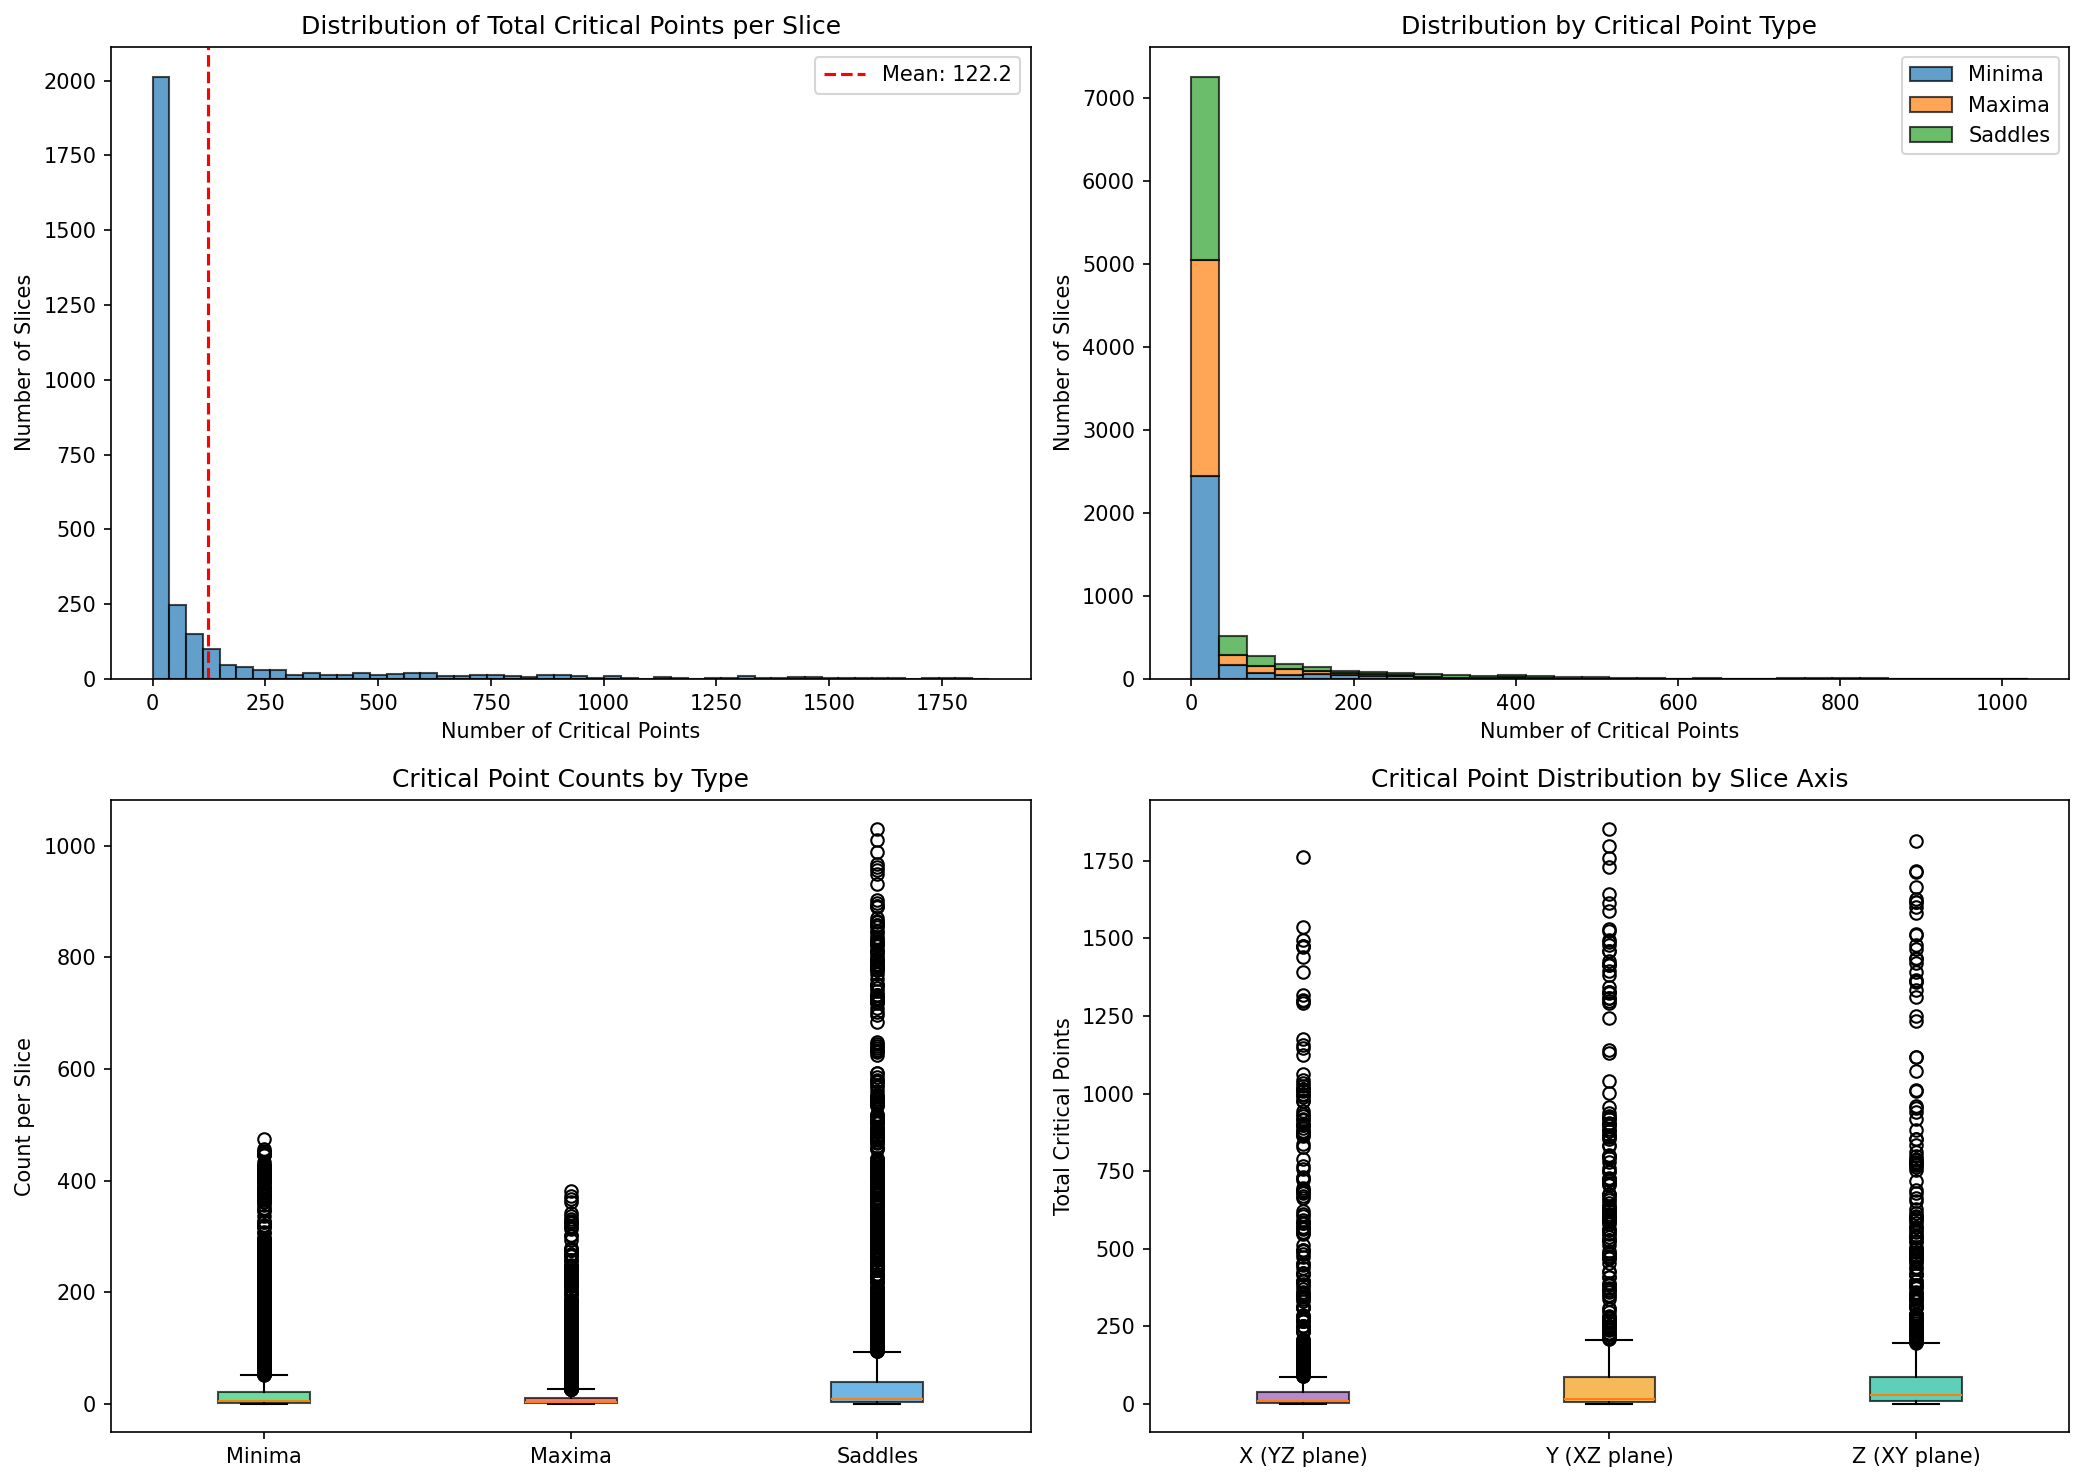
\includegraphics[width=\textwidth]{analysis/critical_points_distribution.png}
%     \caption{Distribution of critical points across slices.}
%     \label{fig:cp-distribution}
% \end{figure}

\subsection{Baseline Methods}

We compare against the following baselines:

\paragraph{SZ Compression}
% TODO: Run SZ experiments and fill in results
\begin{itemize}
    \item Error bounds tested: [TODO]
    \item Results: [TODO]
\end{itemize}

\paragraph{ZFP Compression}
% TODO: Run ZFP experiments and fill in results
\begin{itemize}
    \item Rates tested: [TODO]
    \item Results: [TODO]
\end{itemize}

\paragraph{VAE Baseline}
% TODO: Train VAE and fill in results
\begin{itemize}
    \item Architecture: [TODO]
    \item Results: [TODO]
\end{itemize}

% TODO: Add baseline comparison table
% % TODO: Fill in after running baseline experiments
\begin{table}[h]
\centering
\caption{Comparison of compression methods. CR = Compression Ratio, CPR = Critical Point detection Rate, CPE = Critical Point position Error (pixels).}
\label{tab:baseline-comparison}
\begin{tabular}{lccccc}
\toprule
Method & CR & PSNR (dB) & SSIM & CPR (\%) & CPE \\
\midrule
SZ (eb=1e-3) & -- & -- & -- & -- & -- \\
SZ (eb=1e-4) & -- & -- & -- & -- & -- \\
ZFP (8 bpv) & -- & -- & -- & -- & -- \\
ZFP (16 bpv) & -- & -- & -- & -- & -- \\
VAE (d=128) & -- & -- & -- & -- & -- \\
\midrule
Ours & -- & -- & -- & -- & -- \\
\bottomrule
\end{tabular}
\end{table}


\subsection{Diffusion Model Results}

% TODO: Train diffusion model and fill in results

\paragraph{Training}
\begin{itemize}
    \item Architecture: [TODO]
    \item Training iterations: [TODO]
    \item Training time: [TODO]
\end{itemize}

\paragraph{Reconstruction Quality}
% TODO: Add results

\paragraph{Critical Point Preservation}
% TODO: Add results

\subsection{RL Agent Results}

% TODO: Train RL agent and fill in results

\paragraph{Policy Behavior}
% TODO: Analyze learned policy

\paragraph{Compression Performance}
% TODO: Add results

\paragraph{Comparison with Baselines}
% TODO: Add comparison table and figures

\subsection{Ablation Studies}

% TODO: Run ablation studies

\paragraph{Reward Function Components}
% TODO: Ablate different reward terms

\paragraph{Architecture Choices}
% TODO: Ablate architecture decisions


% Section 6: Lessons Learned
\section{Lessons Learned and Future Work}
\label{sec:conclusion}

% Q6: What did we learn? What other problems could this apply to? How could it be improved?

\subsection{Key Insights}

% TODO: Fill in after experiments complete

From our experiments, we learned:

\begin{enumerate}
    \item \textbf{[TODO: Insight 1]}

    \item \textbf{[TODO: Insight 2]}

    \item \textbf{[TODO: Insight 3]}
\end{enumerate}

\subsection{Limitations}

Our approach has several limitations:

\begin{itemize}
    \item \textbf{Computational cost}: [TODO: Discuss inference time]
    \item \textbf{Training requirements}: [TODO: Discuss data and compute needs]
    \item \textbf{Generalization}: [TODO: Discuss domain transfer]
\end{itemize}

\subsection{Future Work}

Several directions could extend this work:

\paragraph{Multi-field Compression}
Scientific simulations often produce multiple correlated fields (density, velocity, temperature). Joint compression could exploit cross-field correlations.

\paragraph{3D Extension}
Our current work uses 2D slices for tractability. Extending to full 3D volumes would enable richer topological analysis but requires addressing computational challenges.

\paragraph{Time-Series Compression}
Temporal coherence in simulation sequences could be exploited for better compression of time-varying data.

\paragraph{Real-Time In-Situ Compression}
Integrating the compression policy into simulation codes could enable real-time data reduction during computation.

\paragraph{Other Domains}
The approach could potentially transfer to:
\begin{itemize}
    \item Climate and weather data
    \item Medical imaging (CT, MRI)
    \item Fluid dynamics simulations
\end{itemize}

\subsection{Conclusion}

% TODO: Write conclusion after experiments complete

We presented [TODO: summary of contribution]. Our experiments on NYX cosmology data demonstrate [TODO: key results]. This work opens new directions for task-aware scientific data compression that preserves semantically important features.

\paragraph{Broader Impact}
Improved scientific data compression could enable:
\begin{itemize}
    \item Larger simulations within storage constraints
    \item Faster data sharing in scientific collaborations
    \item Better archival of long-term scientific campaigns
\end{itemize}


\bibliographystyle{plain}
\bibliography{bibliography}

\end{document}
